\documentclass{beamer}
\usetheme{Singapore}
%\setbeamercolor{structure}{fg=red}
\usepackage{upgreek}
\usepackage{color}
%\def\magyarOptions{hyphenation=huhyphn}
%\usepackage{ae,aecompl}
%\usepackage[T1]{fontenc}
\usepackage[utf8]{inputenc}
%\usepackage[hungarian]{babel}
\usepackage{gensymb}
\usepackage{pgfplots}
\usepackage{pst-plot}
\usepackage{tikz}
\usepgfplotslibrary{external}
\tikzexternalize
\usepackage[version=3]{mhchem}
\usepackage{listings}

\normalfont
\title{Deconvolution in Scanning Electrochemical Microscopy}
\author
{
Dr. András Kiss\\
}

\institute
{
  %\inst{1}%
  Department of General and Physical Chemistry\\
  University of Pécs, Hungary\\
    \hfill \\

  \includegraphics[width=0.14\textwidth]{pte_logo.eps}\\
  \vspace{0.1cm}
  Center for Integrative Physiology\\
  and Molecular Medicine\\
  Universität des Saarlandes, Homburg, Germany
  
  \includegraphics[width=0.2\textwidth]{cipmm.png}\\

  %June 16, 2017
}

\date[]

\begin{document}
%\frame{\titlepage}  


\begin{frame}[plain]
        \centering
        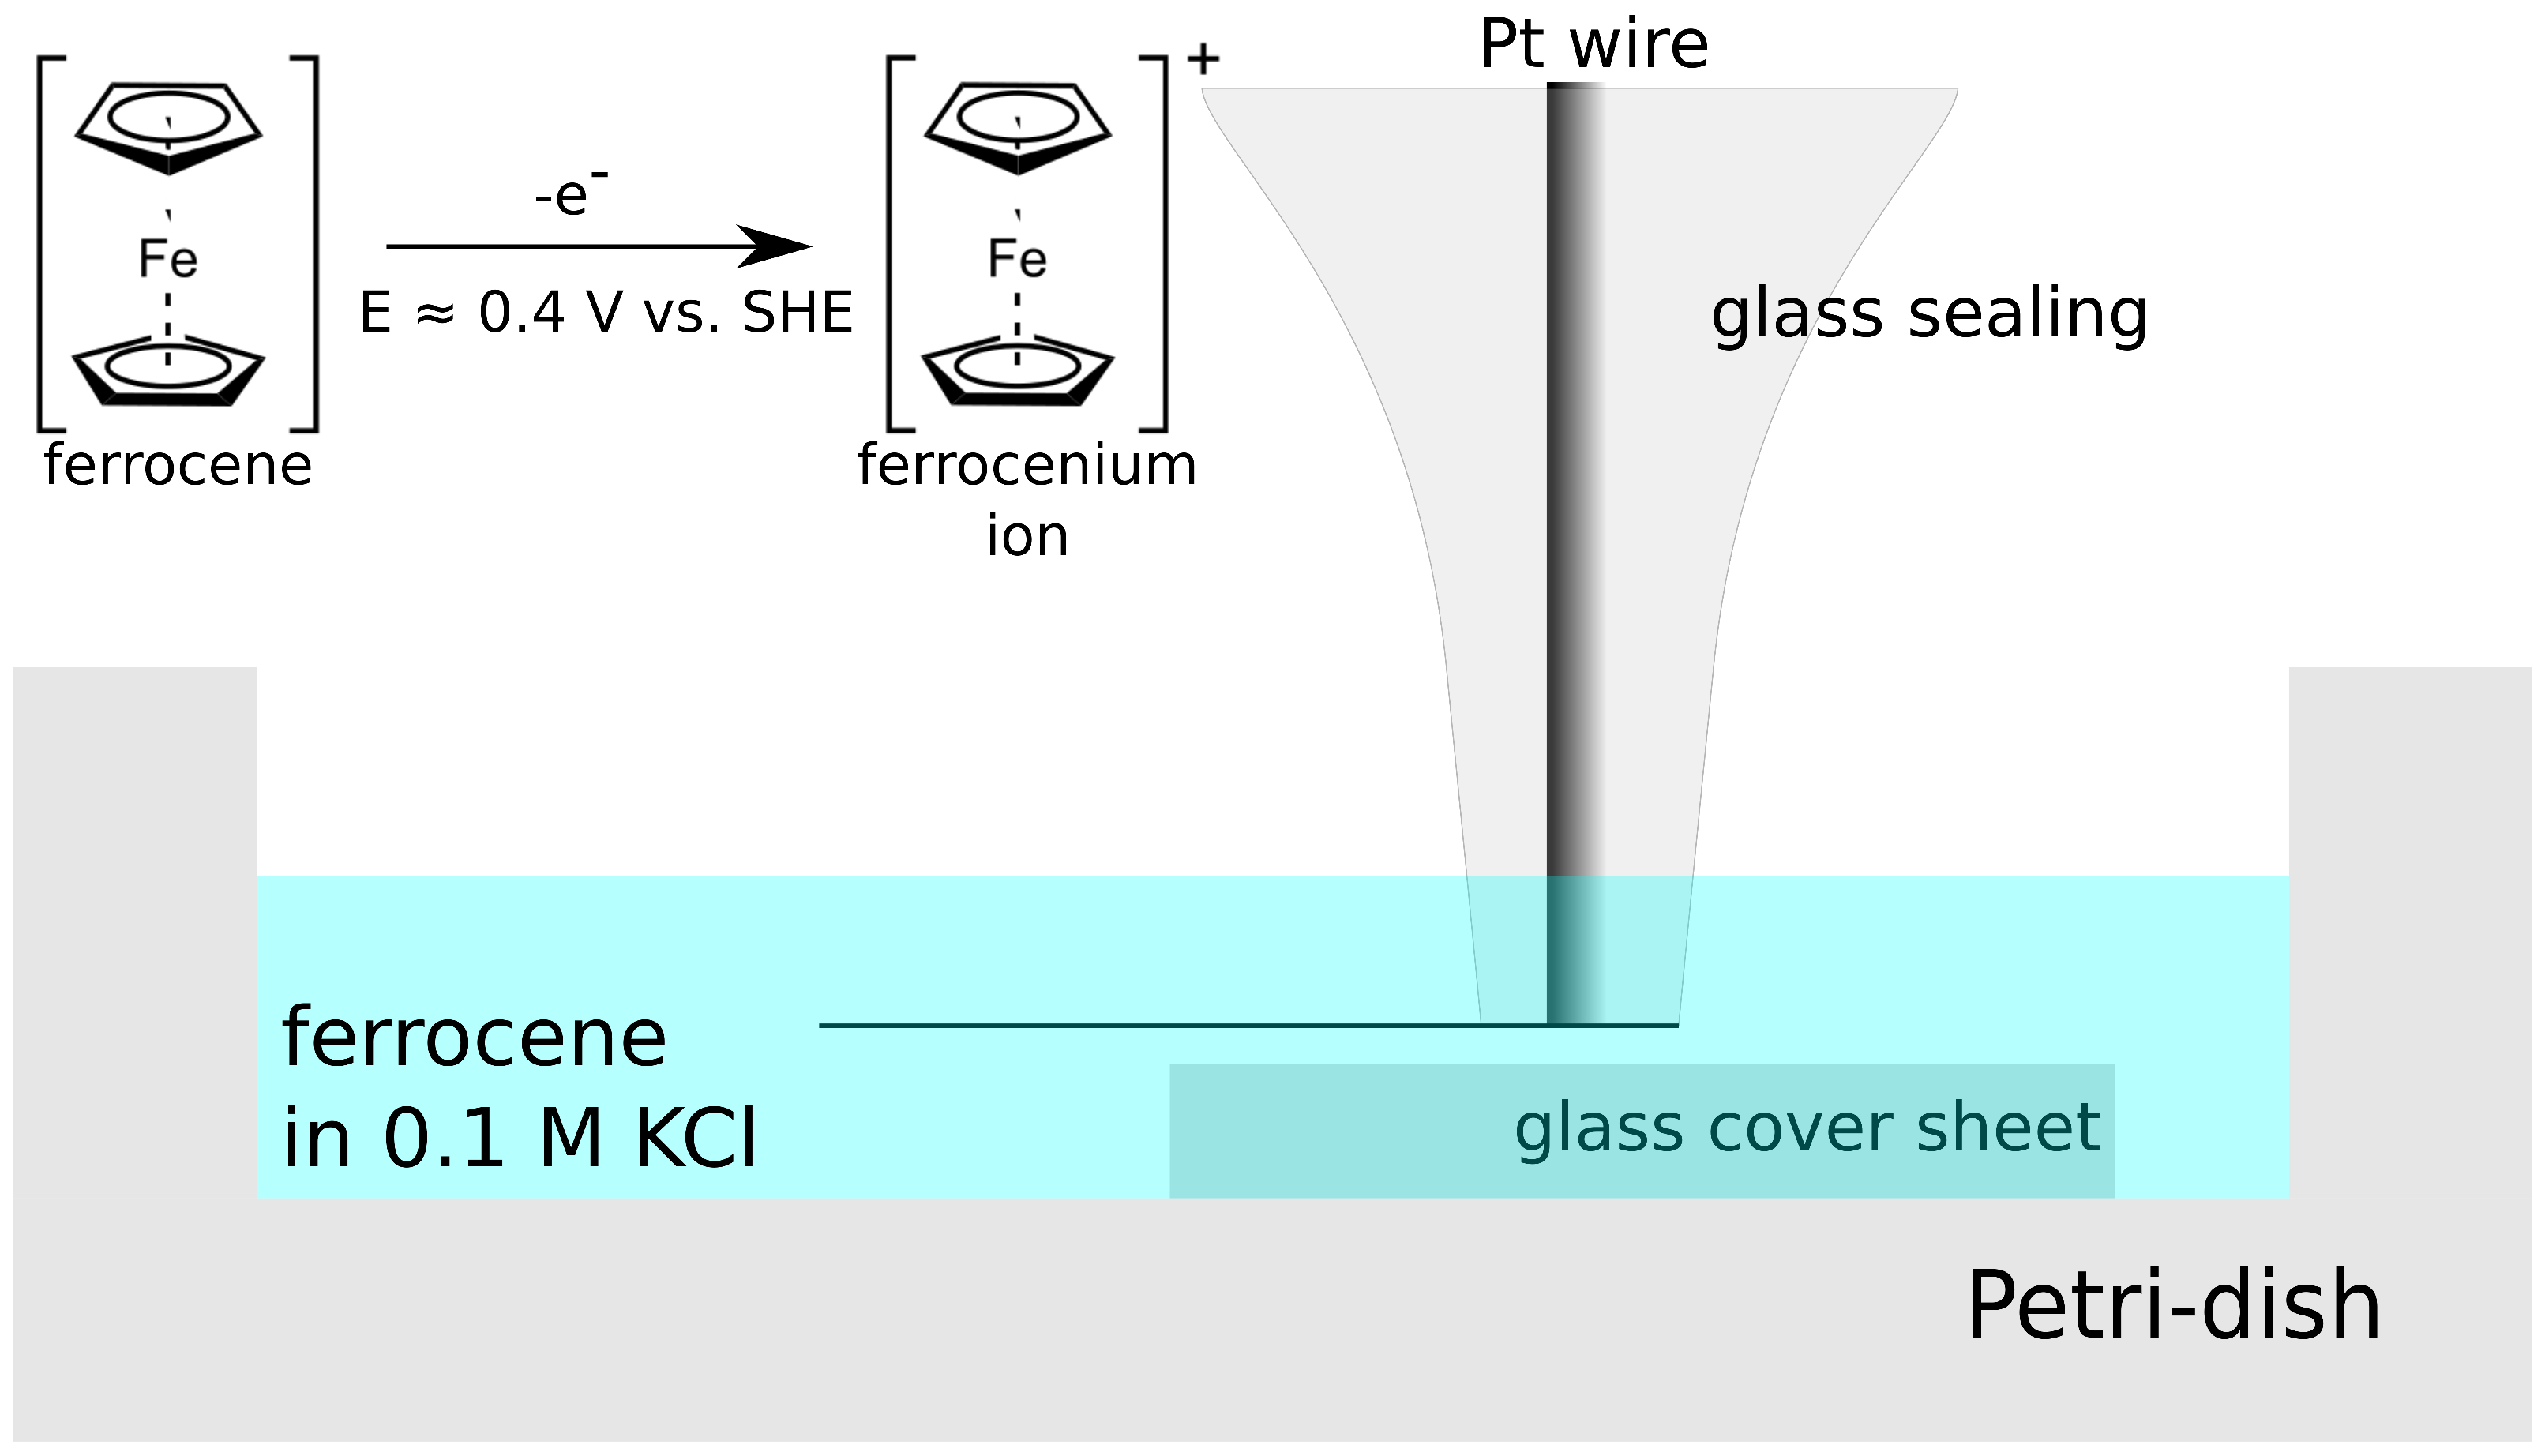
\includegraphics[width=0.4\textwidth]{step.eps}
\vfill
\end{frame}

\begin{frame}[plain]

        \centering
        \includegraphics[trim = 10mm 60mm 0mm 60mm, clip, width=0.33\textwidth, angle=-90]{1.eps}\includegraphics[trim = 10mm 60mm 0mm 60mm, clip, width=0.33\textwidth, angle=-90]{2_meandered.eps}\includegraphics[trim = 10mm 60mm 0mm 60mm, clip, width=0.33\textwidth, angle=-90]{2_meandered_deconvoluted.eps}

\hspace{1.2cm} 5 $\upmu$m/s \hspace{1.2cm} 10 $\upmu$m/s \hspace{0.2cm} 10 $\upmu$m/s deconvoluted \hfill
\vfill
\end{frame}

\begin{frame}[plain]

        \centering
        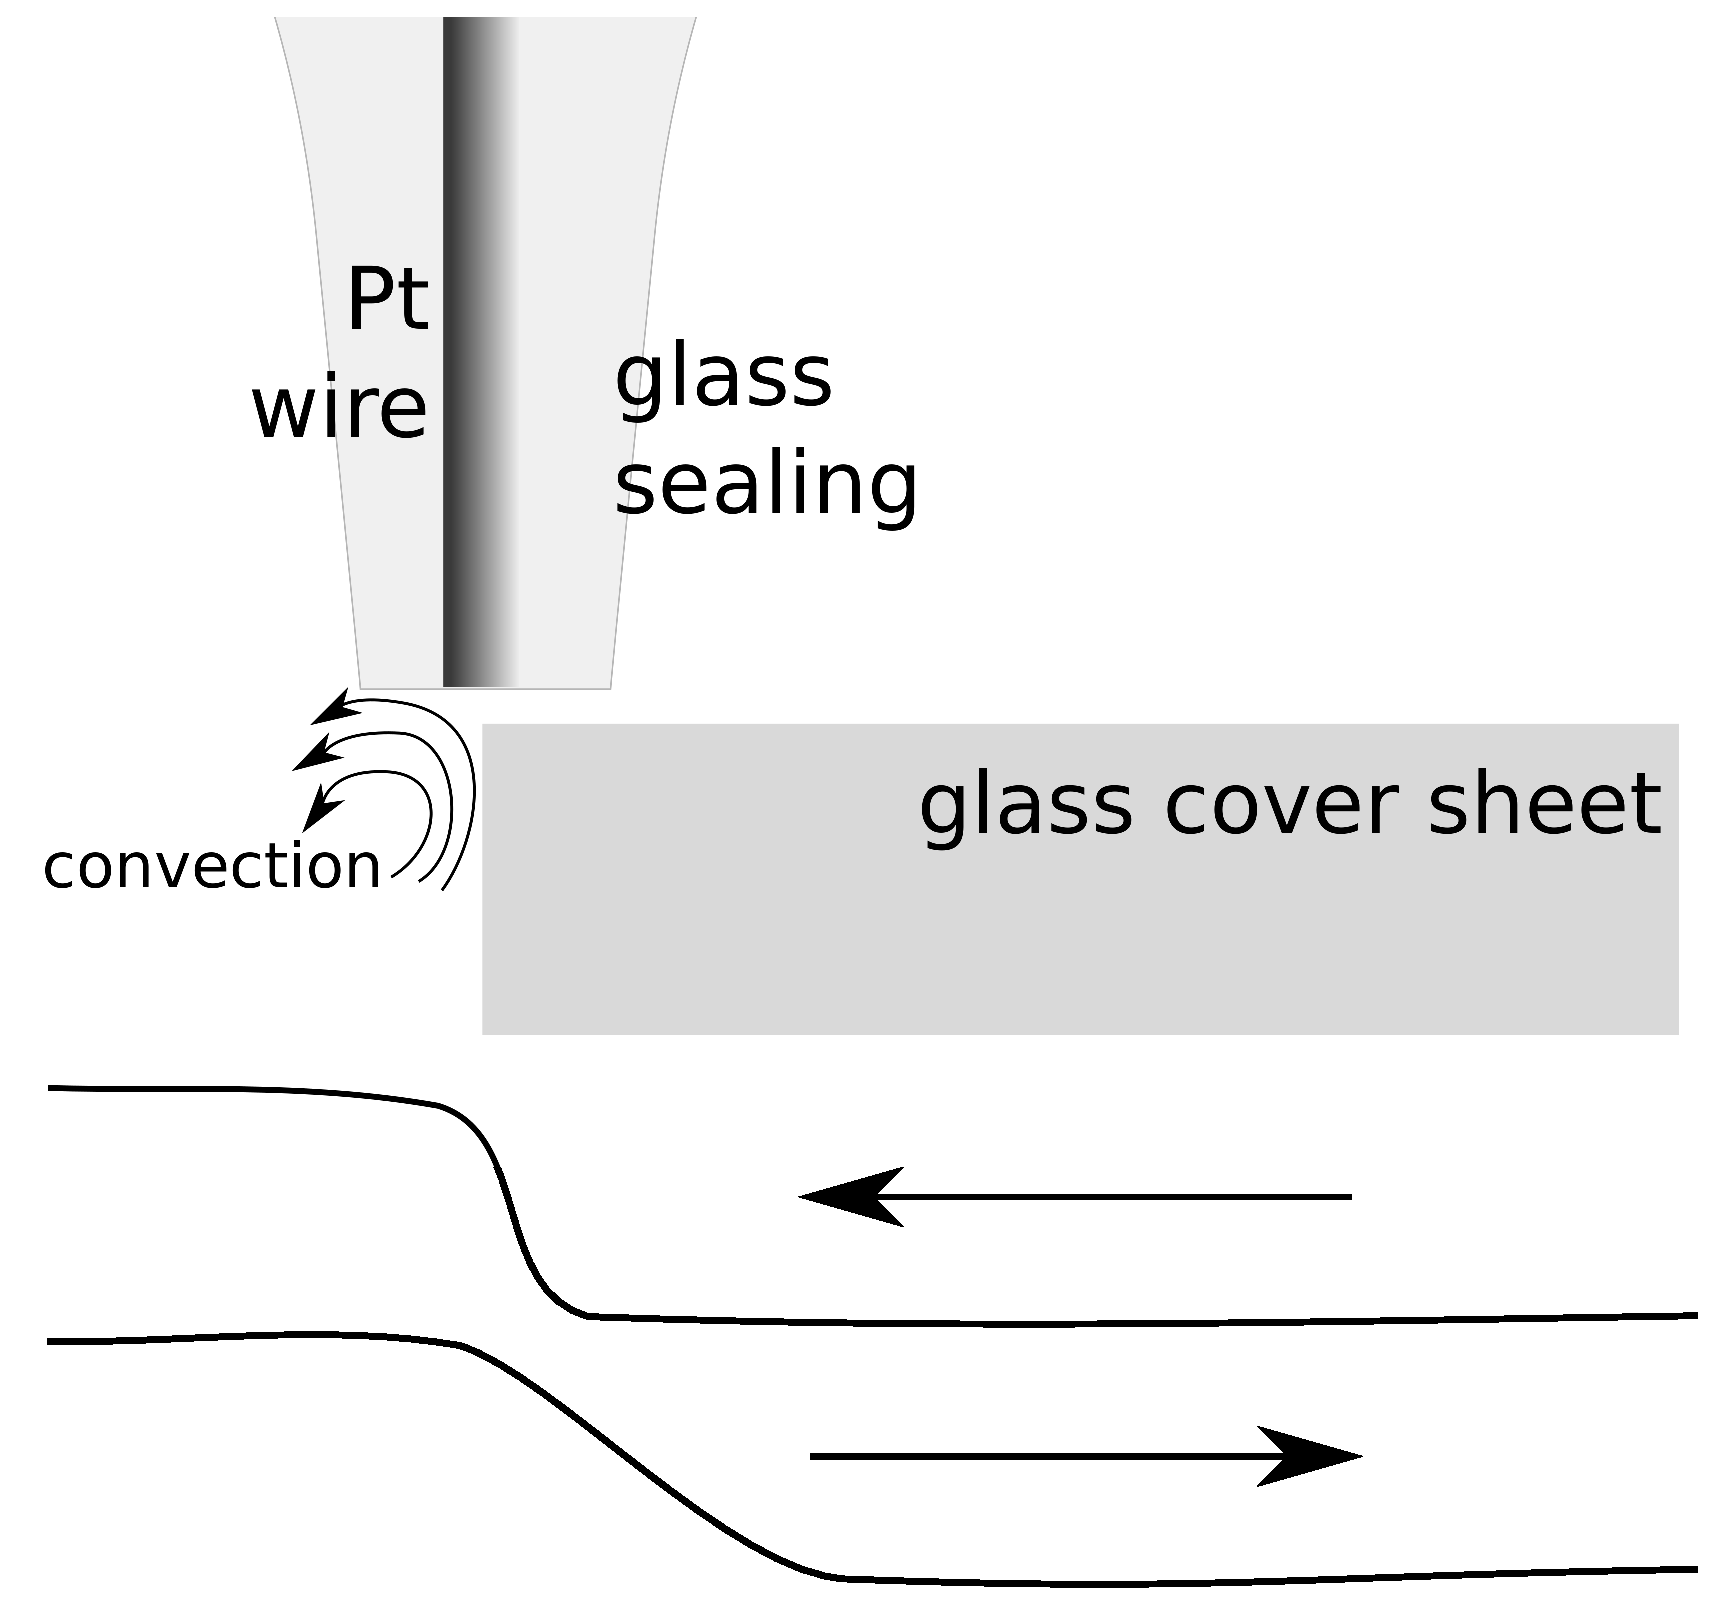
\includegraphics[width=0.4\textwidth]{step_conv.eps}
\vfill
\end{frame}


\begin{frame}[plain]

        \centering
        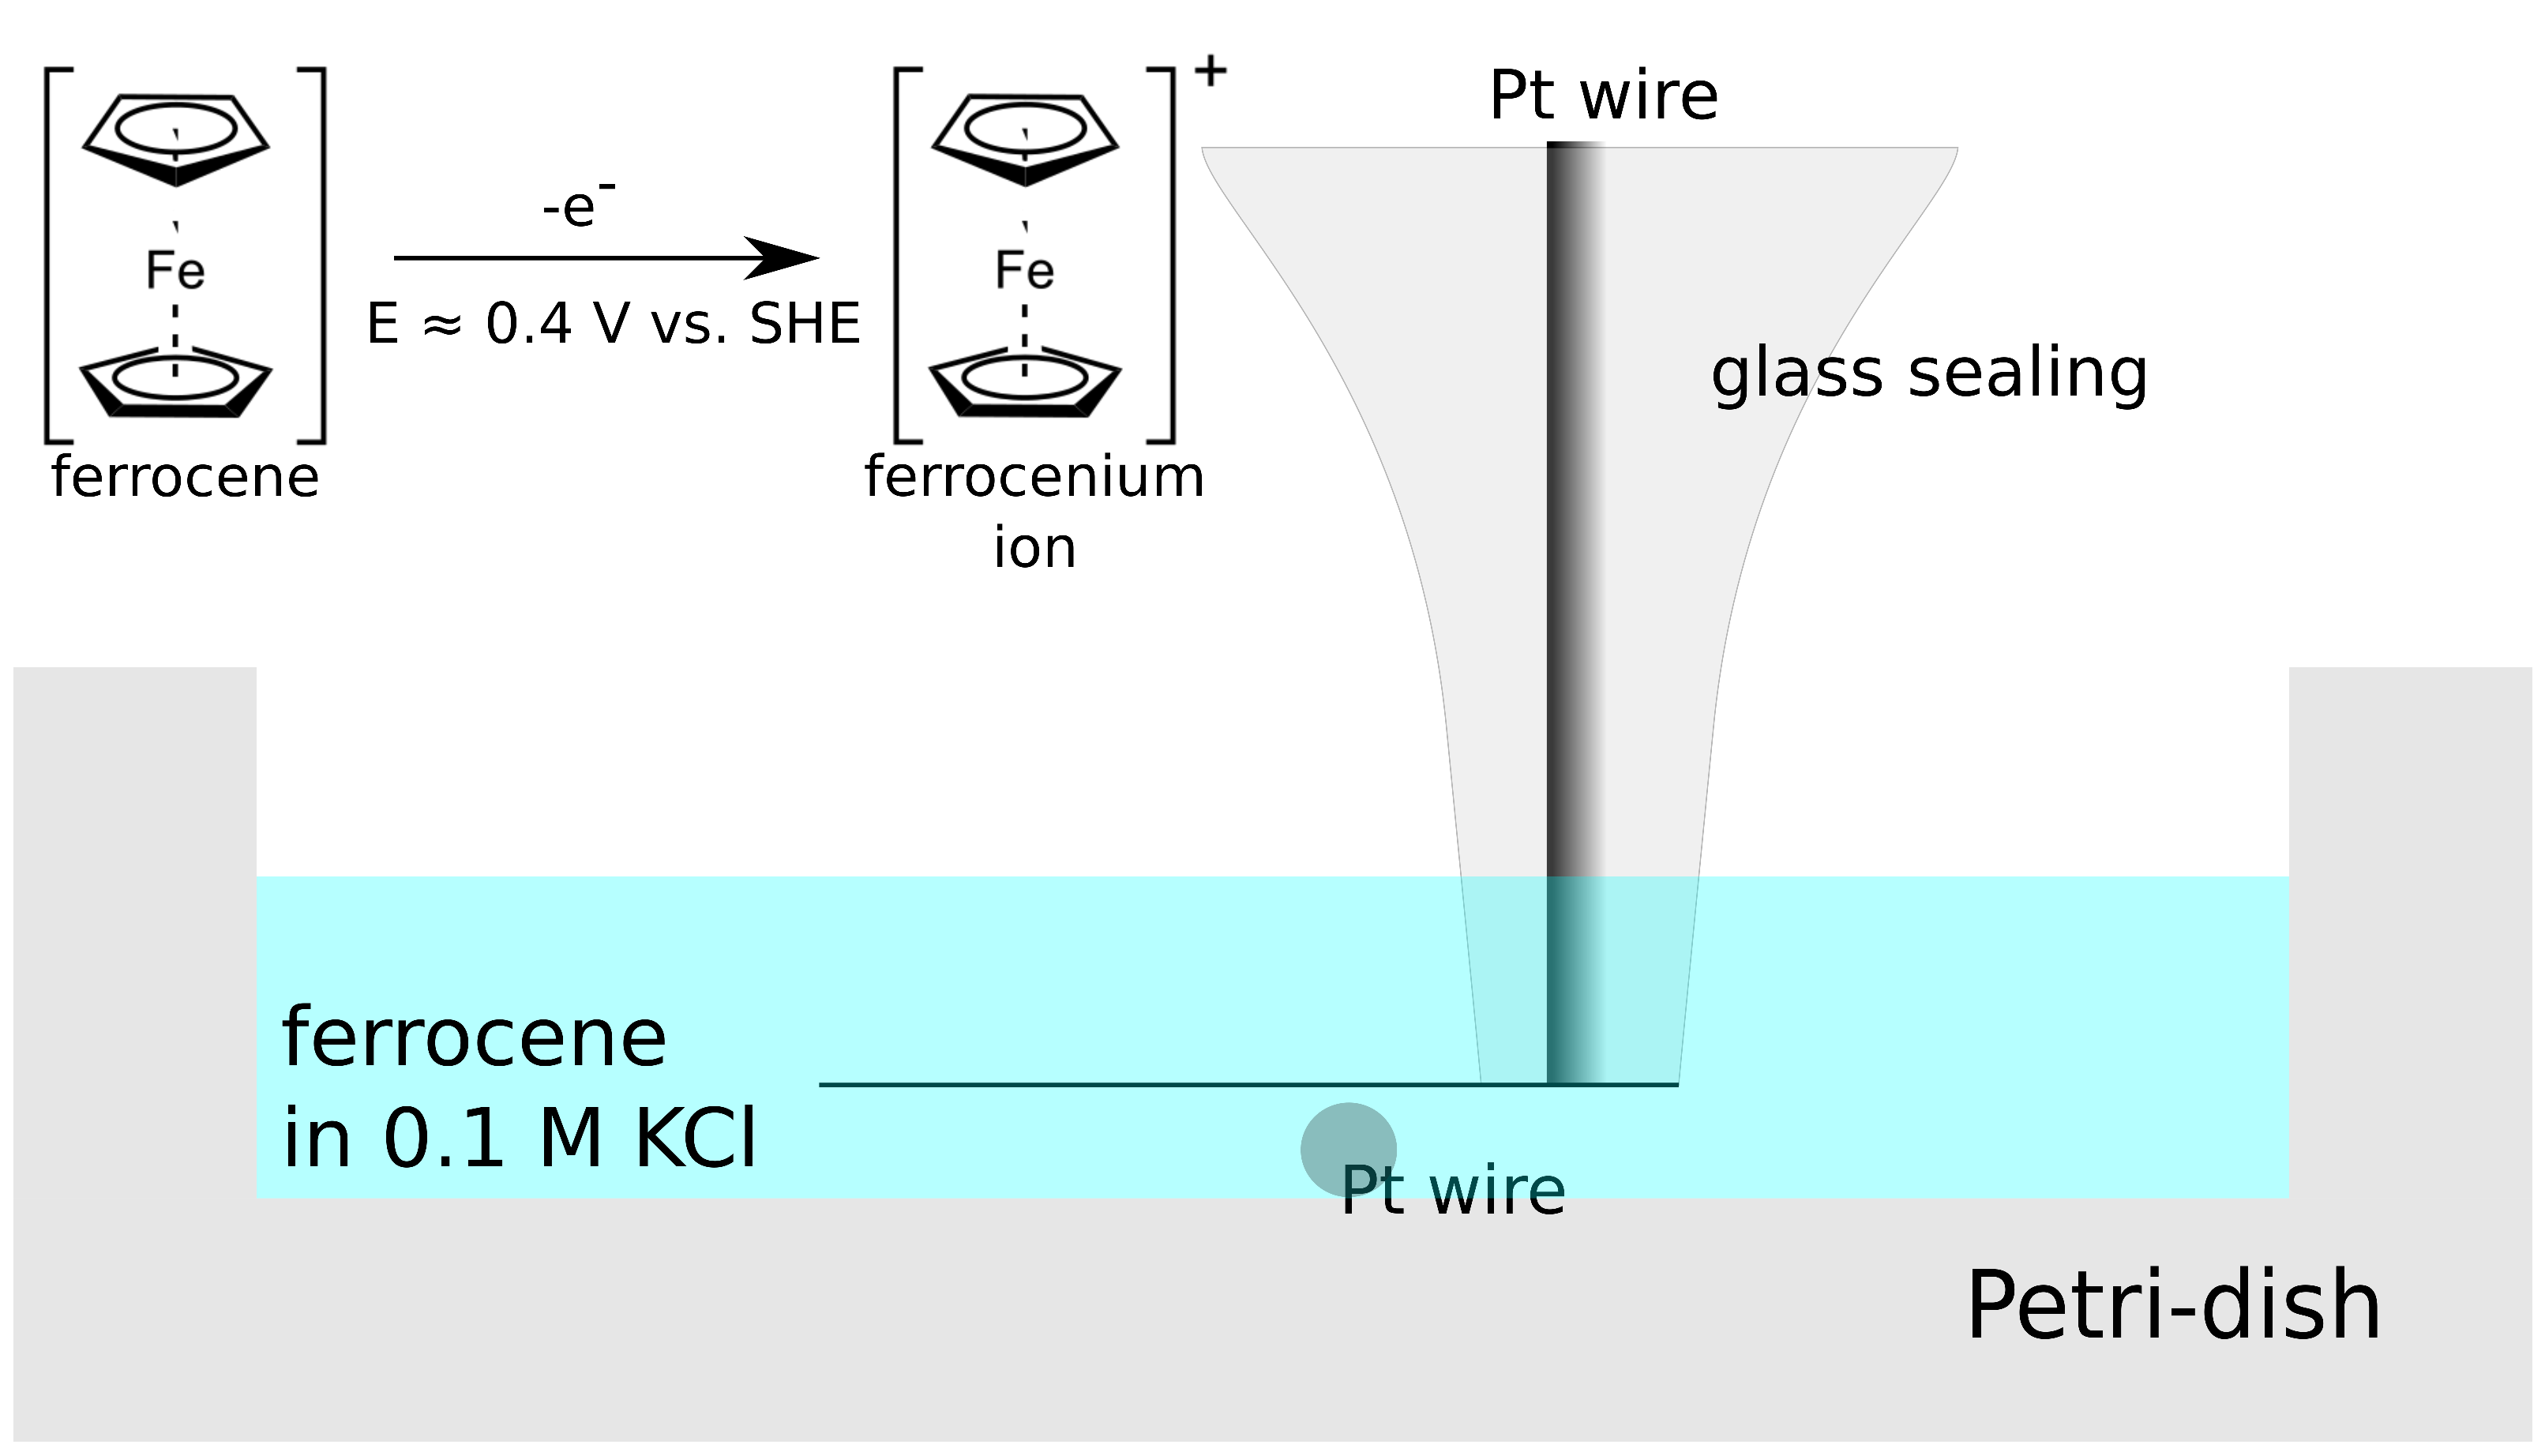
\includegraphics[width=0.4\textwidth]{wire.eps}
\vfill
\end{frame}

\begin{frame}[plain]

        \centering
        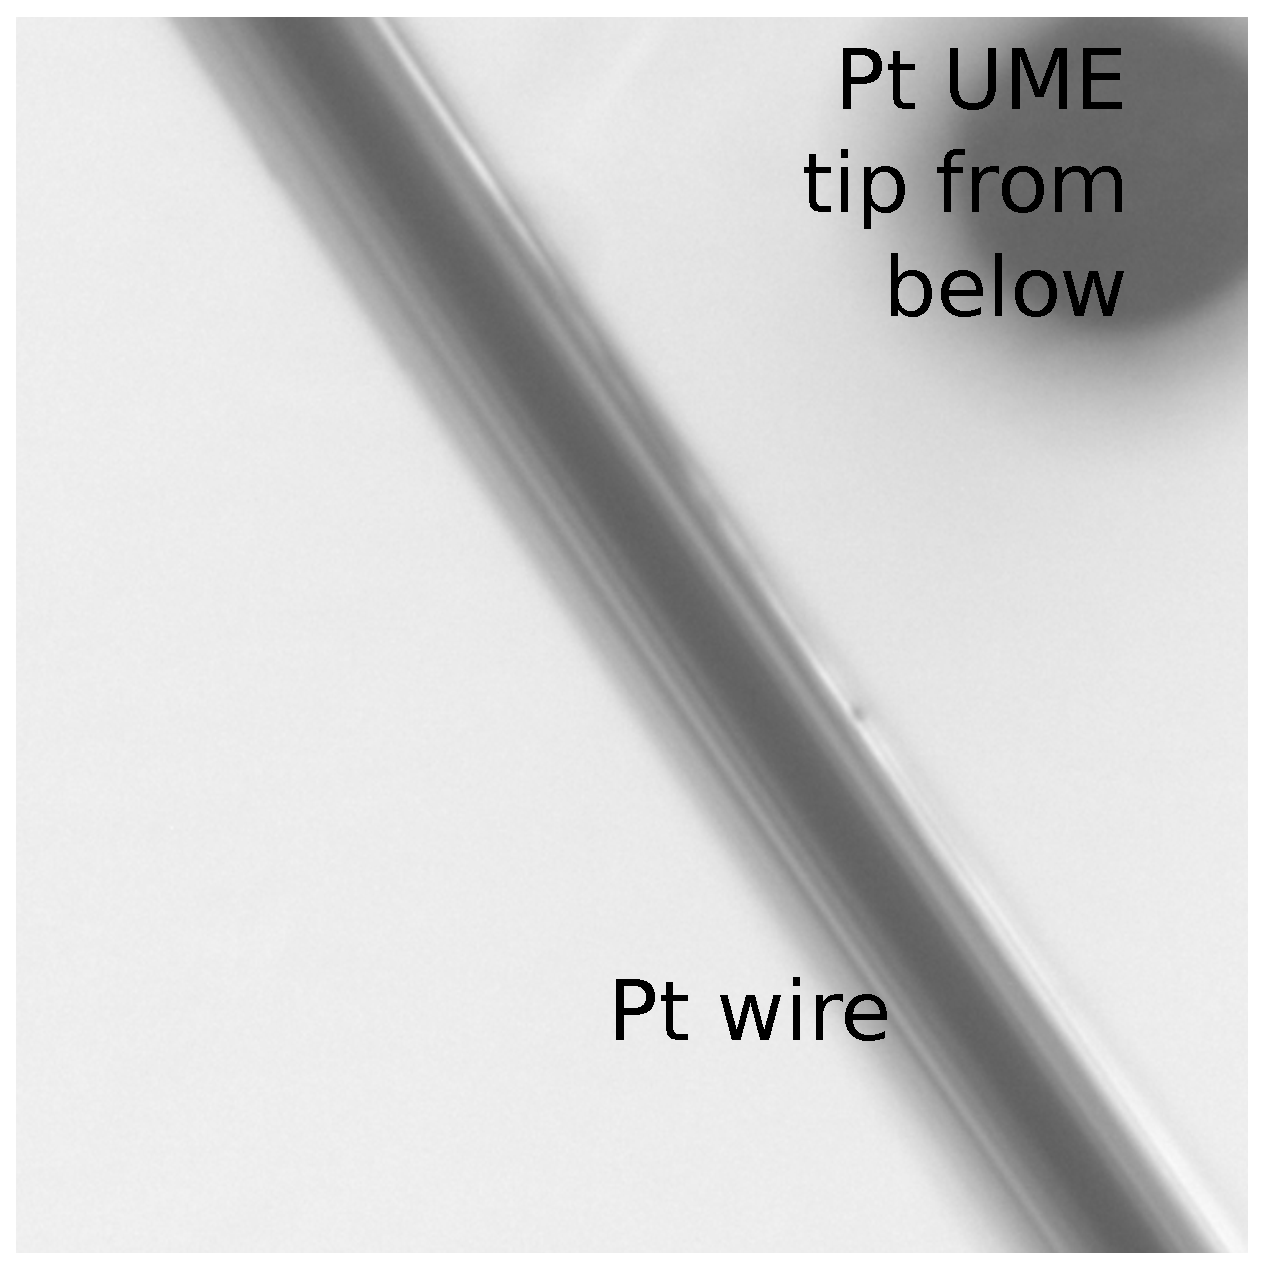
\includegraphics[width=0.4\textwidth]{wire_photo.eps}
\vfill
\end{frame}


\begin{frame}[plain]

        \centering
        \includegraphics[trim = 10mm 10mm 0mm 10mm, clip, width=0.4\textwidth, angle=-90]{7.eps}\includegraphics[trim = 10mm 30mm 0mm 10mm, clip, width=0.4\textwidth, angle=-90]{7_deconvoluted.eps}

\hspace{1.4cm} 10 $\upmu$m/s \hspace{3cm} 10 $\upmu$m/s deconvoluted

\vfill
\end{frame}


\begin{frame}[plain]

        \centering
        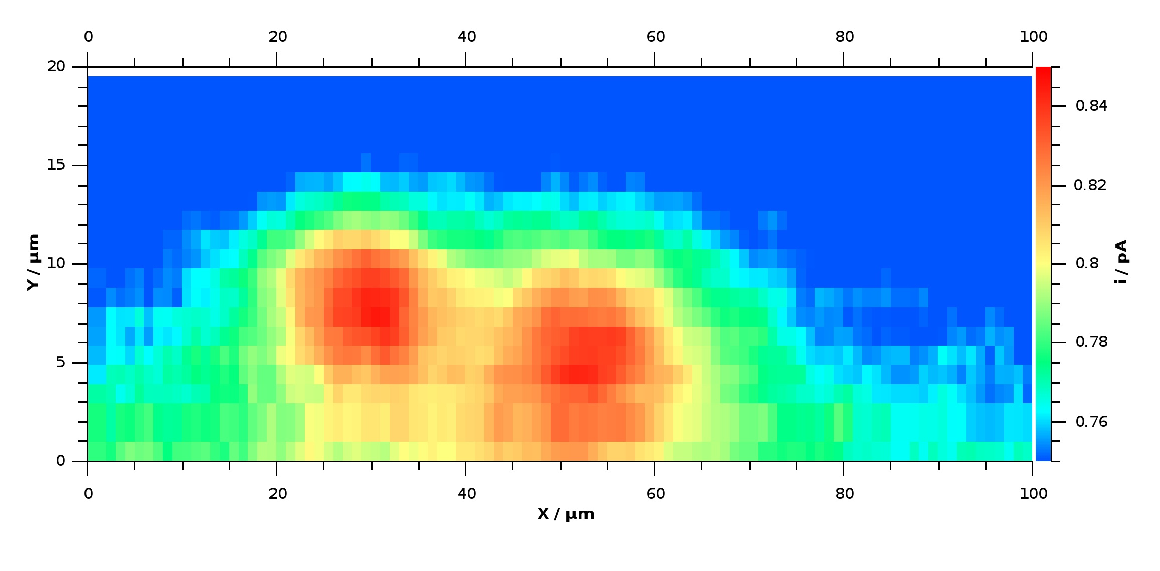
\includegraphics[width=0.4\textwidth]{original.eps}
	
	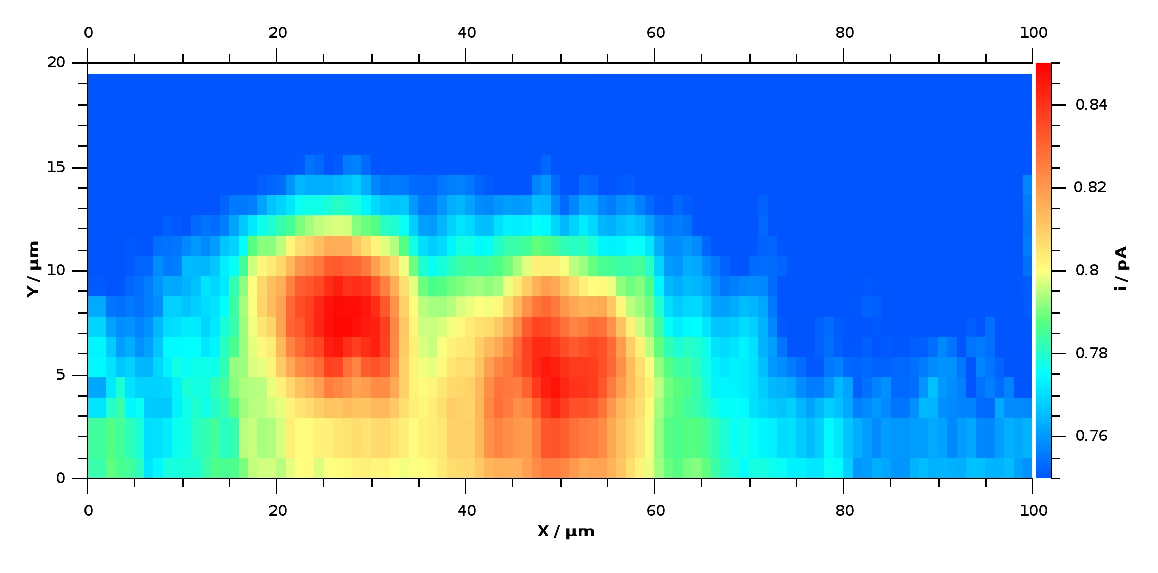
\includegraphics[width=0.4\textwidth]{deconvoluted.eps}

%\hspace{1.2cm} 5 $\upmu$m/s \hspace{1.2cm} 10 $\upmu$m/s \hspace{0.2cm} 10 $\upmu$m/s deconvoluted \hfill


\vfill
\end{frame}


\begin{frame}[plain]

        \centering
        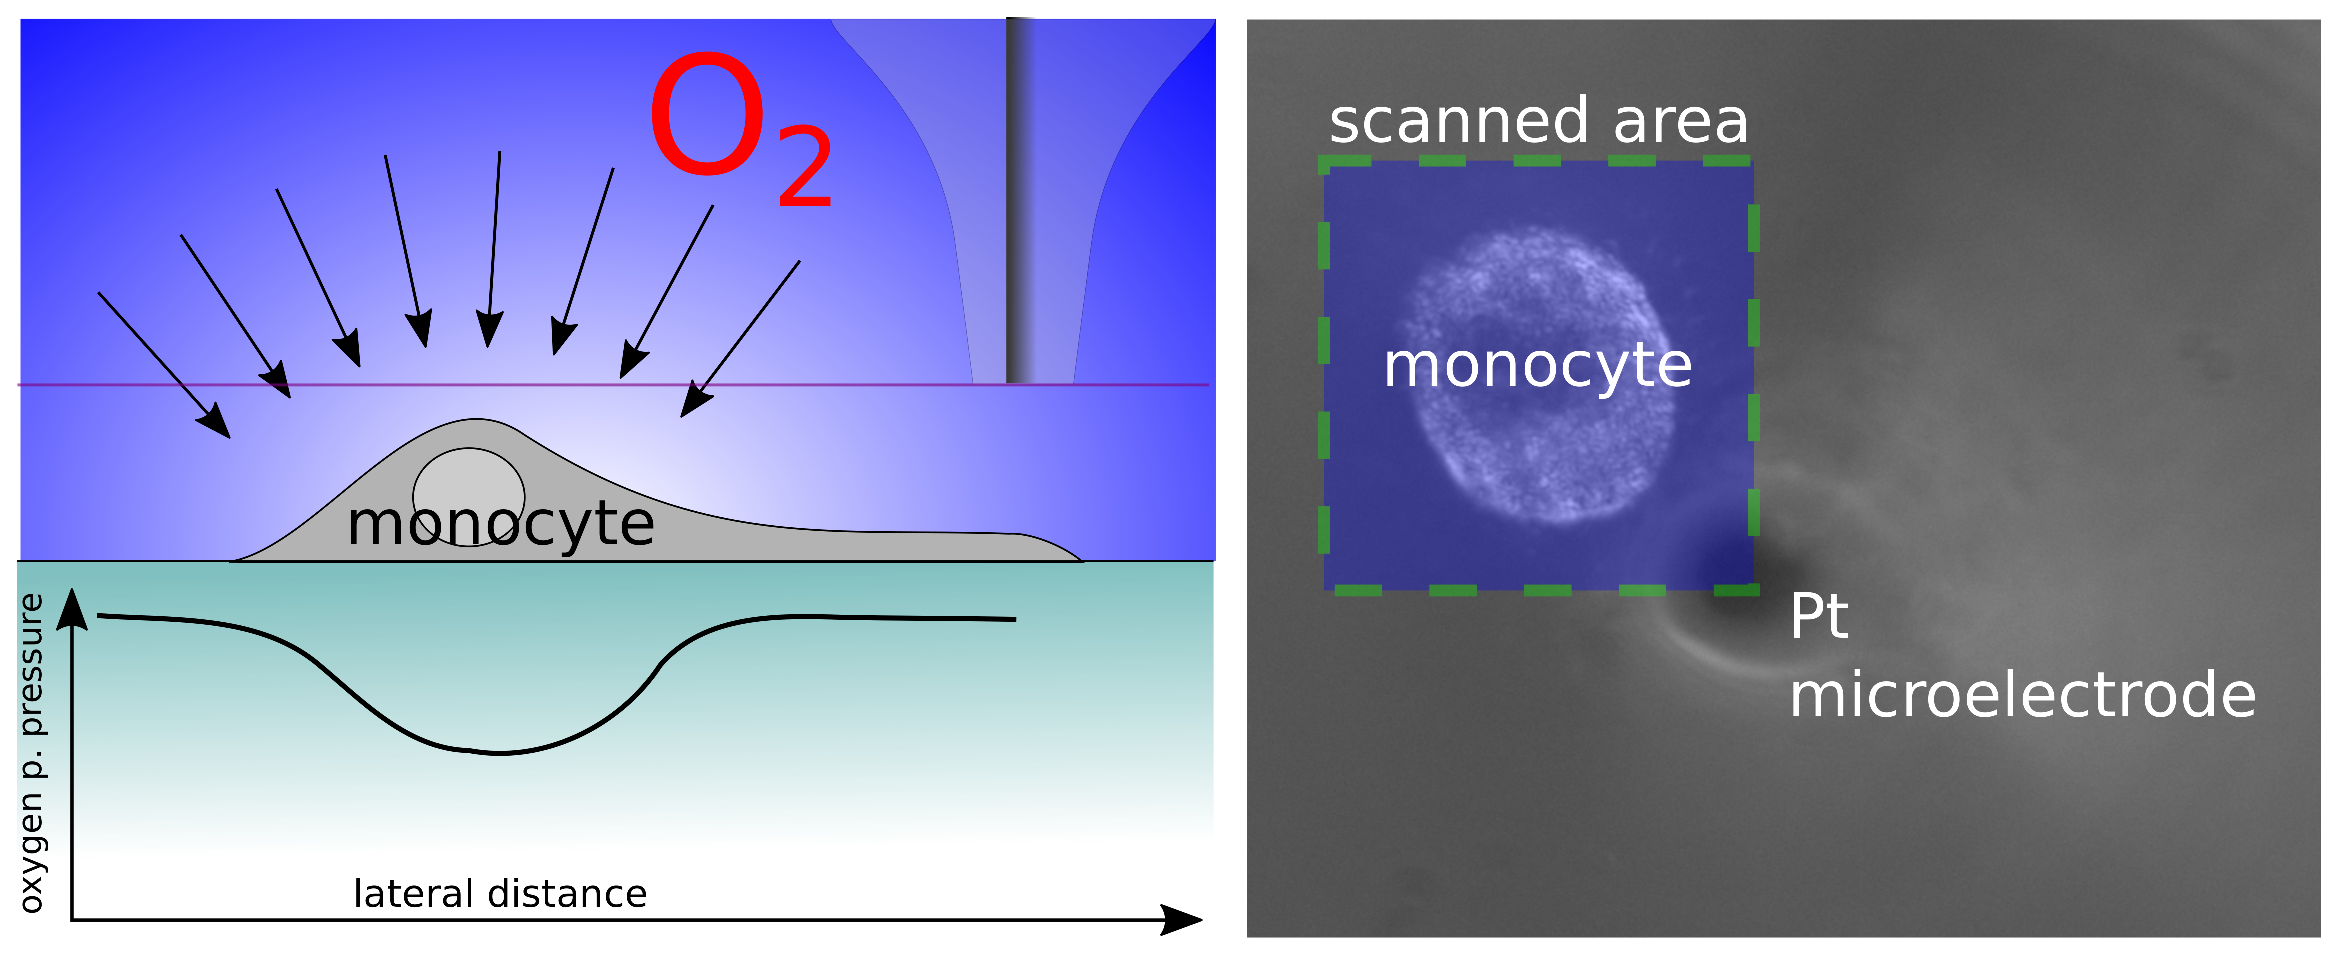
\includegraphics[width=0.7\textwidth]{oxygen.eps}

\end{frame}


\begin{frame}[plain]

        \centering
        \includegraphics[trim = 10mm 20mm 0mm 20mm, clip, width=0.3\textwidth, angle=-90]{9_41.eps}\includegraphics[trim = 10mm 20mm 0mm 20mm, clip, width=0.3\textwidth, angle=-90]{9_41_meandered_deconvoluted.eps}

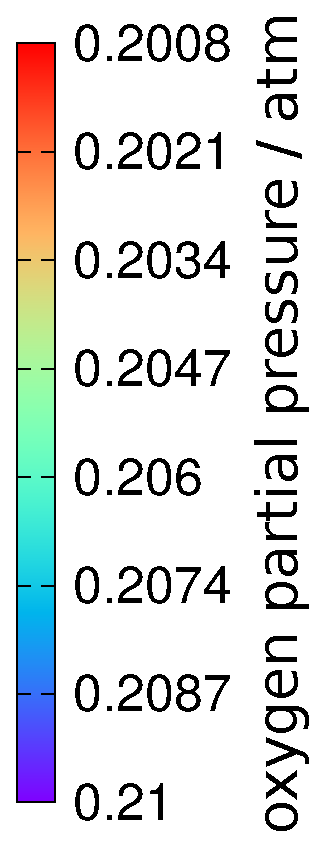
\includegraphics[width=0.1\textwidth, angle=-90]{atm.eps}

%\hspace{1.2cm} 5 $\upmu$m/s \hspace{1.2cm} 10 $\upmu$m/s \hspace{0.2cm} 10 $\upmu$m/s deconvoluted \hfill

\vfill
\end{frame}




\end{document}
